\section{CAPÍTULO I: Información de la empresa}

\subsection{Razón social}

\begin{description}
	\item[Nombre de empresa:] CESTYS - PERU E.I.R.L.
	\item[RUC:] 20600604733
	\item[Dirección:] AV.Independencia  N°257 
	\item[Gerente General:] GAMION ESPEJO GUDELIA YADHIRA
	\item[Sector:] Privado
	\item[Actividades Económicas:] Principal - 8530 - ENSEÑANZA SUPERIOR
\end{description}
\begin{figure}
	\centering
	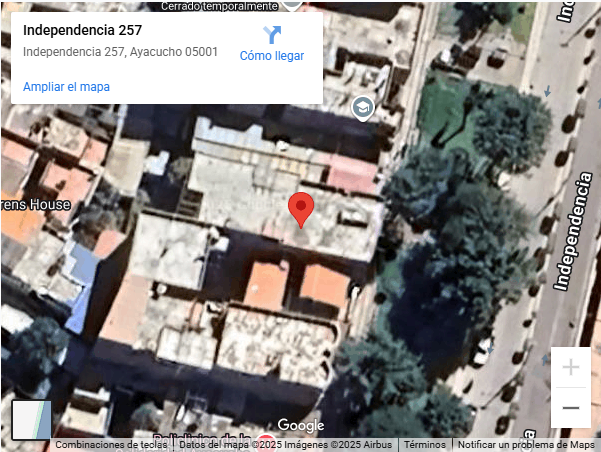
\includegraphics[width=0.7\linewidth]{Figuras/11-08-08-2025-11}
	\caption{Dirección de la empresa CESTYS - PERU E.I.R.L.}
	\label{fig:11-08-08-2025-11}
\end{figure}



\subsection{Misión, Visión, Objetivos, Valores de la empresa}


\subsubsection{Misión}
Brindar programas de capacitación en Tecnología, Gestión Pública, Ingeniería, Arquitectura y Salud, con una metodología práctica y actualizada, que permita a nuestros estudiantes adquirir las habilidades necesarias para insertarse en el mundo laboral en corto tiempo, impulsando así su desarrollo personal y profesional.

\subsubsection{Visión}
Ser reconocidos a nivel nacional como una institución líder en formación técnica y profesional de corta duración, que transforma vidas al facilitar el acceso rápido al empleo y promover la continuidad de estudios superiores.

\subsubsection{Objetivo general}
Formar profesionales competentes en un periodo de 2, 4 o 6 meses, capaces de responder a las demandas del mercado laboral y generar oportunidades para el crecimiento educativo y económico de nuestros egresados.

\subsubsection{Valores}
\begin{itemize}
	\item \textbf{Compromiso:} Trabajamos con dedicación para garantizar la calidad de la enseñanza y el éxito de nuestros estudiantes.
	\item \textbf{Excelencia:} Mantenemos altos estándares académicos y profesionales.
	\item \textbf{Innovación:} Incorporamos metodologías y contenidos actualizados según las tendencias del mercado.
	\item \textbf{Responsabilidad:} Cumplimos con nuestra labor educativa con ética y transparencia.
	\item \textbf{Trabajo en equipo:} Fomentamos la colaboración entre docentes, personal y alumnos para alcanzar objetivos comunes.
\end{itemize}



\subsection{Productos, mercado, clientes}
\subsubsection{Productos}
Los productos de esta institución educativa son servicios de formación y capacitación profesional, no objetos físicos. La oferta académica está diseñada para brindar conocimientos y habilidades relevantes, permitiendo a los estudiantes mejorar su perfil profesional y personal. La empresa se dedica a enseñar y capacitar en diversas áreas de alta demanda.

\begin{itemize}
	\item \textbf{Programas de capacitación:}
	
	\begin{itemize}
		\item Administración y gestión empresarial (Cajero Financiero y Comercial, Contabilidad y Finanzas, etc).
		\item Ciencias de la salud (Asistente de farmacia, Asistente dental, Asistente en fisioterapia y rehabilitación).
		\item Gestión pública (Administración pública, políticas públicas).
		\item Ingeniería y arquitectura (Topografía, Lectura de planos, etc).
		\item Tecnología e informática ( Ofimatica, Edicion y postproduccion de videos, etc).
	\end{itemize}
	
	
	\item \textbf{Modalidades de estudio:} Presencial y virtual, ofreciendo flexibilidad y accesibilidad para diferentes perfiles de estudiantes.
\end{itemize}

\subsubsection{Mercado}
El mercado para esta institución está determinado por factores como ubicación, demanda y competencia.

\begin{itemize}
	\item \textbf{Ubicación geográfica:} Principalmente en Ayacucho, con alcance nacional e internacional gracias a la modalidad virtual.
	\item \textbf{Tamaño del mercado:} Jóvenes de 17 a 25 años y profesionales que buscan formación continua.
	\item \textbf{Tendencias:} Aumento de la demanda de educación virtual y especializada, impulsada por la digitalización y necesidades del mercado laboral.
	\item \textbf{Competencia:} Universidades e institutos (públicos y privados), que compiten en calidad académica, infraestructura, costos y prestigio.
\end{itemize}

\subsubsection{Clientes}
Los principales clientes son los estudiantes, quienes se agrupan en dos grandes segmentos:

\paragraph{Estudiantes de pregrado}
\begin{itemize}
	\item \textbf{Demografía:} Jóvenes recién egresados de secundaria (17 a 25 años).
	\item \textbf{Motivación:} Obtener un título profesional, mejorar su calidad de vida y contribuir a su comunidad.
	\item \textbf{Necesidades:} Educación de calidad, tecnología, apoyo académico, orientación, costos accesibles, empleabilidad.
\end{itemize}

\paragraph{Estudiantes de posgrado y educación continua}
\begin{itemize}
	\item \textbf{Demografía:} Profesionales mayores de 25 años, activos en el mercado laboral.
	\item \textbf{Motivación:} Especializarse, ascender, cambiar de carrera o actualizar conocimientos.
	\item \textbf{Necesidades:} Flexibilidad, modalidad virtual, contenido actualizado, docentes con experiencia, red de contactos.
\end{itemize}

\subsection{Estructura de la Organización}
\subsection{Otra información relevante de la empresa donde se desarrolla el proyecto}

% CAPÍTULO II
